\documentclass{standalone}
\usepackage{tikz}

\begin{document}
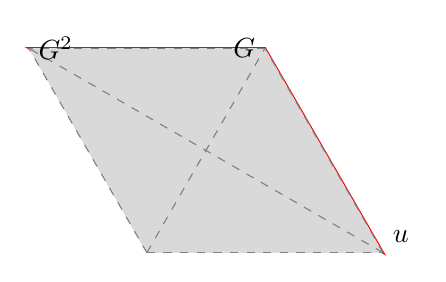
\begin{tikzpicture}[scale=3]

% Define points
\coordinate (O) at (0,0);
\coordinate (u) at (1,0);
\coordinate (G) at (0.5,0.866);
\coordinate (G2) at (-0.5,0.866);

% Draw convex hull
\draw[red, thick] (u) -- (G) -- (G2) -- cycle;

% Draw ruled-out regions in grey
\fill[gray!30] (O) -- (u) -- (G) -- cycle;
\fill[gray!30] (O) -- (u) -- (G2) -- cycle;
\fill[gray!30] (O) -- (G) -- (G2) -- cycle;

% Draw lines to indicate ruled-out regions
\draw[dashed, gray] (O) -- (u);
\draw[dashed, gray] (O) -- (G);
\draw[dashed, gray] (O) -- (G2);
\draw[dashed, gray] (u) -- (G);
\draw[dashed, gray] (u) -- (G2);
\draw[dashed, gray] (G) -- (G2);

% Label points
\node[above right] at (u) {$u$};
\node[left] at (G) {$G$};
\node[right] at (G2) {$G^2$};

\end{tikzpicture}
\end{document}